\begin{frame}{¿Qué se ve en el STM?}
    \begin{block}{Nota importante}
        En STM la imagen no es una fotografía directa de la superficie. 
        Es una reconstrucción de la señal de túnel, sensible tanto a la geometría como a la densidad local de estados electrónicos.
    \end{block}

    \vspace{2mm}

\end{frame}




\begin{frame}{¿Qué se ve en el STM?}

    \begin{itemize}
        \item El factor de transmision decae aproximadamente como $T \sim e^{-2\kappa}z, \quad \kappa \approx \sqrt{2m\phi/\hbar^{2}}$.
        
        \item El contraste depende del voltaje, la corriente de setpoint y el estado de la punta.
        \item La interpretación correcta requiere separar efectos topográficos, electrónicos e instrumentales.
    \end{itemize}
\begin{figure}
    \centering
    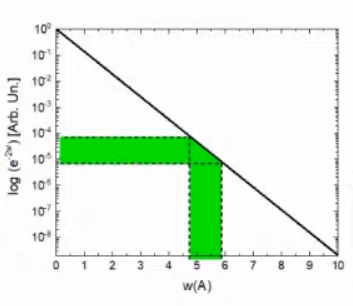
\includegraphics[width=0.4\linewidth]{./images/image.png}
    \caption{Corriente tunel vs Distancia muestra}
    \label{fig:placeholder}
\end{figure}
\end{frame}












\begin{frame}{Imagen en modo de corriente constante}
    En este modo, el lazo de realimentación ajusta la posición vertical de la punta para mantener constante la corriente de túnel.

\begin{figure}
    \centering
    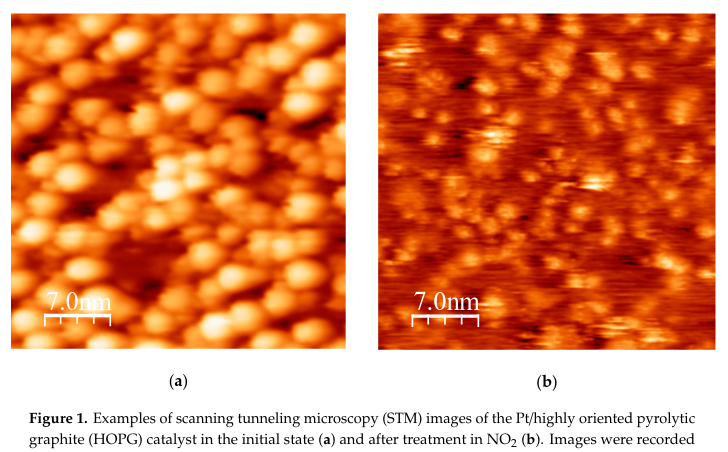
\includegraphics[width=0.6\linewidth]{./images/dddd.png}    
\end{figure}
\end{frame}


\begin{frame}{Imagen en modo de corriente constante}
 \vspace{2mm}
    \begin{itemize}
        \item Ventaja: mayor estabilidad y seguridad para la punta.
        \item Limitación: la imagen mezcla relieve físico y contraste electrónico.
        \item Interpretación: una protrusión aparente puede deberse a mayor densidad de estados.
    \end{itemize}
\end{frame}



\begin{frame}{Imagen en modo de altura constante}
    La punta se mantiene a distancia fija y se mide la variación de la corriente.


    
    \begin{figure}
    \centering
    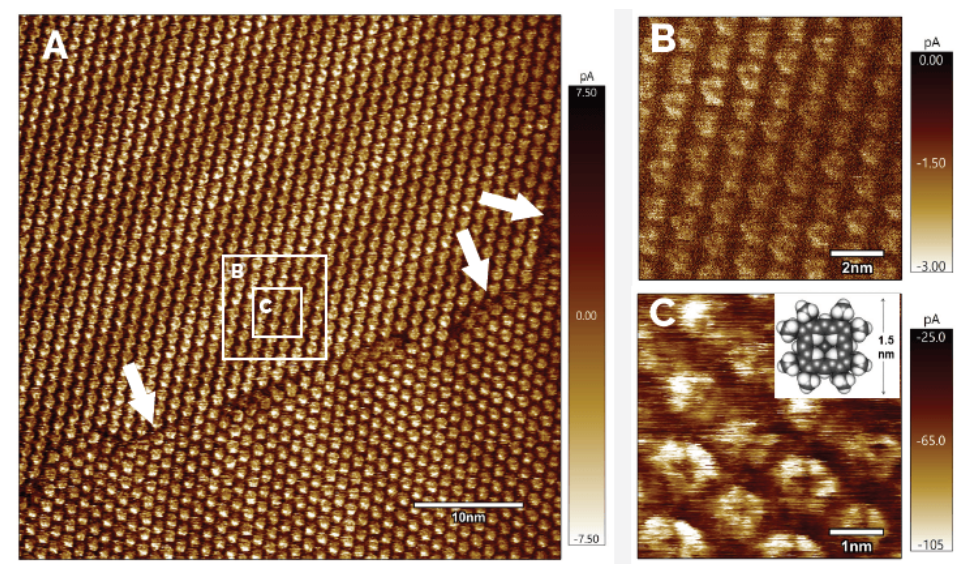
\includegraphics[width=0.5\linewidth]{./images/imagae.png}
    \caption{Constant height STM current images of the 2D lattice of NiOEP on HOPG (highly-oriented pyrolytic graphite ).(A) 50 nm survey scan showing the NiOEP grain boundary (white arrows), zoom regions, and moiré pattern imaged with a 6.4 pA setpoint. (B) Zoomed 10 nm region imaged at 300 fA setpoint. (C) Zoomed 5 nm region showing sub-nm molecular resolution imaged with a 60 pA setpoint. Inset: the CPK molecular model of NiOEP.}
    \label{fig:placeholder}
\end{figure}
\end{frame}





\begin{frame}{Imagen en modo de altura constante}
    \begin{itemize}
        \item Modo más sensible a cambios locales de la muestra.
        \item Requiere superficies muy planas y condiciones muy estables.
        \item Es más riesgoso: pequeños cambios topográficos pueden modificar fuertemente la corriente.
    \end{itemize}
    
    \vspace{2mm}
    \begin{block}{Comparación}
        Corriente constante: más estable. \\
        Altura constante: más directa en la señal, pero más exigente experimentalmente.
    \end{block}
\end{frame}

\begin{frame}{Origen del contraste en STM}
    El contraste observado puede originarse en varios mecanismos superpuestos:
    \begin{itemize}
        \item Relieve geométrico real de la superficie.
        \item Variaciones locales de la densidad electrónica.
        \item Cambios en la barrera de túnel o función de trabajo efectiva.
        \item Defectos, vacancias, adsorbatos, escalones y bordes.
        \item Reconstrucciones superficiales y anisotropías electrónicas.
    \end{itemize}

    \vspace{2mm}

\end{frame}

\begin{frame}{Parámetros experimentales que modifican la imagen}
    \begin{table}
        \centering
        \begin{tabular}{@{}ll@{}}
            \toprule
            Parámetro & Efecto principal \\ \midrule
            Voltaje de polarización & Selecciona la ventana energética explorada \\
            Corriente de setpoint & Fija la distancia punta-muestra \\
            Estado de la punta & Puede cambiar resolución y artefactos \\
            Temperatura & Afecta ruido, estabilidad y difusión superficial \\
            Distancia punta-muestra & Controla la intensidad del túnel \\ \bottomrule
        \end{tabular}
    \end{table}

    \vspace{1mm}
    Cambiar el bias puede alterar el contraste o incluso invertirlo, porque se están observando estados electrónicos distintos.
\end{frame}

\begin{frame}{¿Qué información se puede extraer?}
    Del análisis de imagen STM pueden obtenerse varios observables físicos:
    \begin{itemize}
        \item Periodicidad de la red superficial.
        \item Separaciones entre escalones atómicos.
        \item Defectos puntuales e impurezas.
        \item Tamaño y orientación de dominios.
        \item Rugosidad aparente.
        \item Reconstrucciones superficiales y simetrías.
    \end{itemize}

    \vspace{2mm}
    Con un análisis adecuado también pueden estimarse orientaciones cristalográficas y longitudes de correlación espacial.
\end{frame}

\begin{frame}{Herramientas de análisis de imagen}
La lectura visual sola no basta: conviene apoyar la interpretación con análisis cuantitativo.
    \begin{itemize}
        \item \textbf{Nivelado y sustracción de fondo:} elimina inclinaciones globales y deriva.
        \item \textbf{Perfiles lineales:} permiten medir separaciones, alturas aparentes y anchura de defectos.
        \item \textbf{Histograma de intensidades:} útil para comparar regiones y contrastes.
        \item \textbf{Transformada de Fourier 2D:} revela periodicidades, simetrías y reconstrucciones.
        \item \textbf{Autocorrelación:} cuantifica orden espacial y rugosidad correlacionada.
    \end{itemize}

    \vspace{2mm}
    
\end{frame}

\begin{frame}{Limitaciones y complicaciones}
    \begin{itemize}
        \item \textbf{Punta no ideal:} una punta contaminada o con varios átomos en el ápice distorsiona la imagen.
        \item \textbf{Deriva térmica y creep piezoeléctrico:} alteran distancias y simetrías aparentes.
        \item \textbf{Ruido mecánico y eléctrico:} degrada resolución y estabilidad.
        \item \textbf{Realimentación mal ajustada:} puede suavizar o distorsionar la señal.
    \end{itemize}

    \vspace{2mm}
\begin{figure}
    \centering
    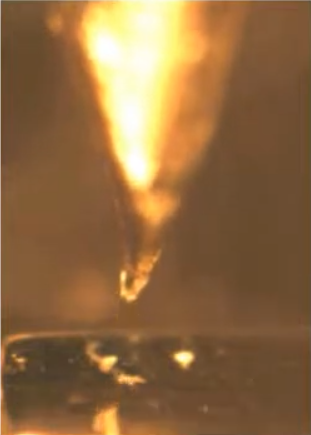
\includegraphics[width=0.2\linewidth]{./images/ffff.png}

\end{figure}

\end{frame}